\documentclass{standalone}
\usepackage{graphicx}	
\usepackage{amssymb, amsmath, amsthm}
\usepackage{color}

\usepackage{tikz}
\usetikzlibrary{math, calc}

\definecolor{light}{RGB}{220, 188, 188}
\definecolor{mid}{RGB}{185, 124, 124}
\definecolor{dark}{RGB}{143, 39, 39}
\definecolor{highlight}{RGB}{180, 31, 180}
\definecolor{lightteal}{RGB}{186, 219, 219}
\definecolor{midteal}{RGB}{124, 186, 186}
\definecolor{darkteal}{RGB}{38, 142, 142}
\definecolor{darkerteal}{RGB}{0, 124, 124}
\definecolor{gray10}{gray}{0.1}
\definecolor{gray20}{gray}{0.2}
\definecolor{gray30}{gray}{0.3}
\definecolor{gray40}{gray}{0.4}
\definecolor{gray60}{gray}{0.6}
\definecolor{gray70}{gray}{0.7}
\definecolor{gray80}{gray}{0.8}
\definecolor{gray90}{gray}{0.9}
\definecolor{gray95}{gray}{0.95}


\begin{document}

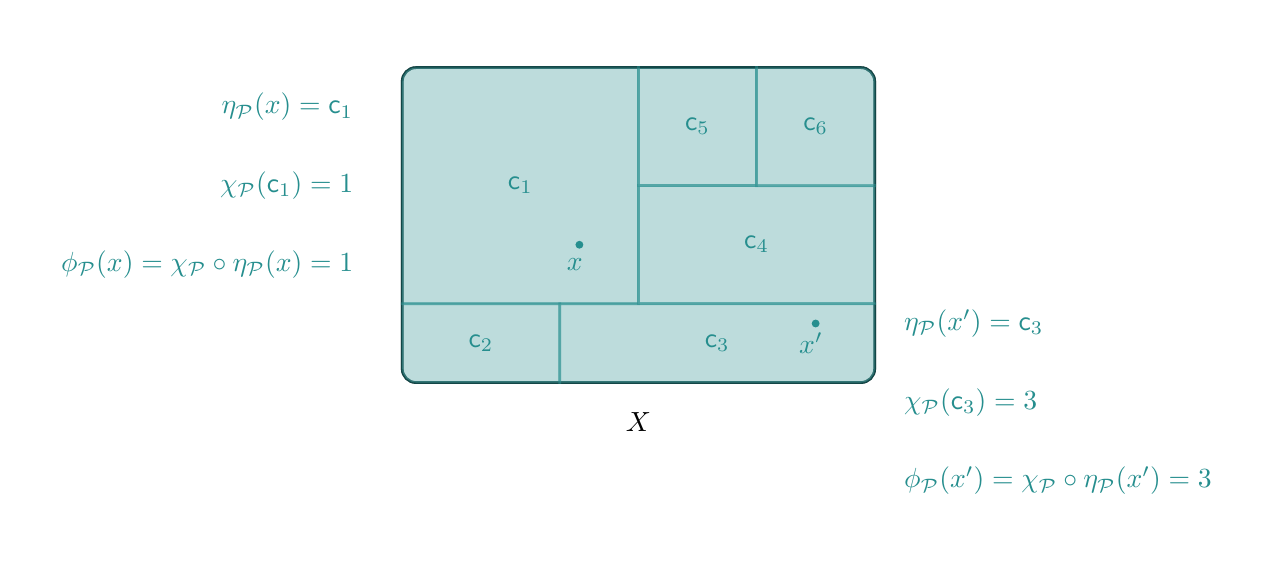
\begin{tikzpicture}[scale=1]
  \draw[white] (-4.75, -2) rectangle (10.75, 4.5);
  \draw[rounded corners=5, color=black, line width=1] (0, 0) rectangle (6, 4);
  \node at (3, -0.5) { $X$ };
  
  \filldraw[draw=darkteal, fill=midteal, opacity=0.5, line width=1]
    (0, 1) -- (3, 1) -- (3, 4) {[rounded corners=5] -- (0, 4)} -- cycle;
  \node[darkteal] at (1.5, 2.5) { $\mathsf{c}_{1}$ };

  \filldraw[draw=darkteal, fill=midteal, opacity=0.5, line width=1]
    (2, 0) -- (2, 1) -- (0, 1) {[rounded corners=5] -- (0, 0)} -- cycle;
  \node[darkteal] at (1, 0.5) { $\mathsf{c}_{2}$ };
  
  \filldraw[draw=darkteal, fill=midteal, opacity=0.5, line width=1]
    (6, 1) -- (2, 1) -- (2, 0) {[rounded corners=5] -- (6, 0)} -- cycle;
  \node[darkteal] at (4, 0.5) { $\mathsf{c}_{3}$ };
  
  \filldraw[draw=darkteal, fill=midteal, opacity=0.5, line width=1] (3, 1) rectangle (6, 2.5);
  \node[darkteal] at (4.5, 1.75) { $\mathsf{c}_{4}$ };
  
  \filldraw[draw=darkteal, fill=midteal, opacity=0.5, line width=1] (3, 2.5) rectangle (4.5, 4);
  \node[darkteal] at (3.75, 3.25) { $\mathsf{c}_{5}$ };
  
  \filldraw[draw=darkteal, fill=midteal, opacity=0.5, line width=1]
    (4.5, 4) -- (4.5, 2.5) -- (6, 2.5) {[rounded corners=5] -- (6, 4)} -- cycle;
  \node[darkteal] at (5.25, 3.25) { $\mathsf{c}_{6}$ };
  
  \fill[darkteal] (2.25, 1.75) circle (0.05);
  \node[darkteal, align=center] at (2.25, 1.5) { $x$ };
  
  \node[darkteal, anchor=east] at (-0.5, 3.5) { $\eta_{\mathcal{P}}(x) = \mathsf{c}_{1}$ };
  \node[darkteal, anchor=east] at (-0.5, 2.5) { $\chi_{\mathcal{P}}(\mathsf{c}_{1}) = 1$ };
  \node[darkteal, anchor=east] at (-0.5, 1.5) 
    { $\phi_{\mathcal{P}}(x) = \chi_{\mathcal{P}} \circ \eta_{\mathcal{P}}(x) = 1$ };
  
  \fill[darkteal] (5.25, 0.75) circle (0.05);
  \node[darkteal, align=center] at (5.25, 0.5) { $x'$ };
  
  \node[darkteal, anchor=west] at (6.25, 0.75) { $\eta_{\mathcal{P}}(x') = \mathsf{c}_{3}$ };
  \node[darkteal, anchor=west] at (6.25, -0.25) { $\chi_{\mathcal{P}}(\mathsf{c}_{3}) = 3$ };
  \node[darkteal, anchor=west] at (6.25, -1.25)
    { $\phi_{\mathcal{P}}(x') = \chi_{\mathcal{P}} \circ \eta_{\mathcal{P}}(x') = 3$ };
    
\end{tikzpicture}

\end{document}  